%!TEX root = ../thesis.tex

\section{シミュレータ}
AI-Formulaのような人の歩行速度以上で移動するロボットは検証する場所を確保することが容易ではないため, アルゴリズムの初期検証などはシミュレータ環境で検証・改善を行うことが望ましい.
AI-Formulaでは基本的な機能が実装されたシミュレータ環境が運営から提供されている.
提供されたシミュレータ環境はモビリティとAIモビリティパーク紫峰の外周コースをシミュレートしたものになっている.
Fig.5.1に提供されたシミュレータ環境の外観を示す.
Fig.5.2にシミュレートするモビリティとコースの外観を示す.

\begin{figure}[H]
  \centering
 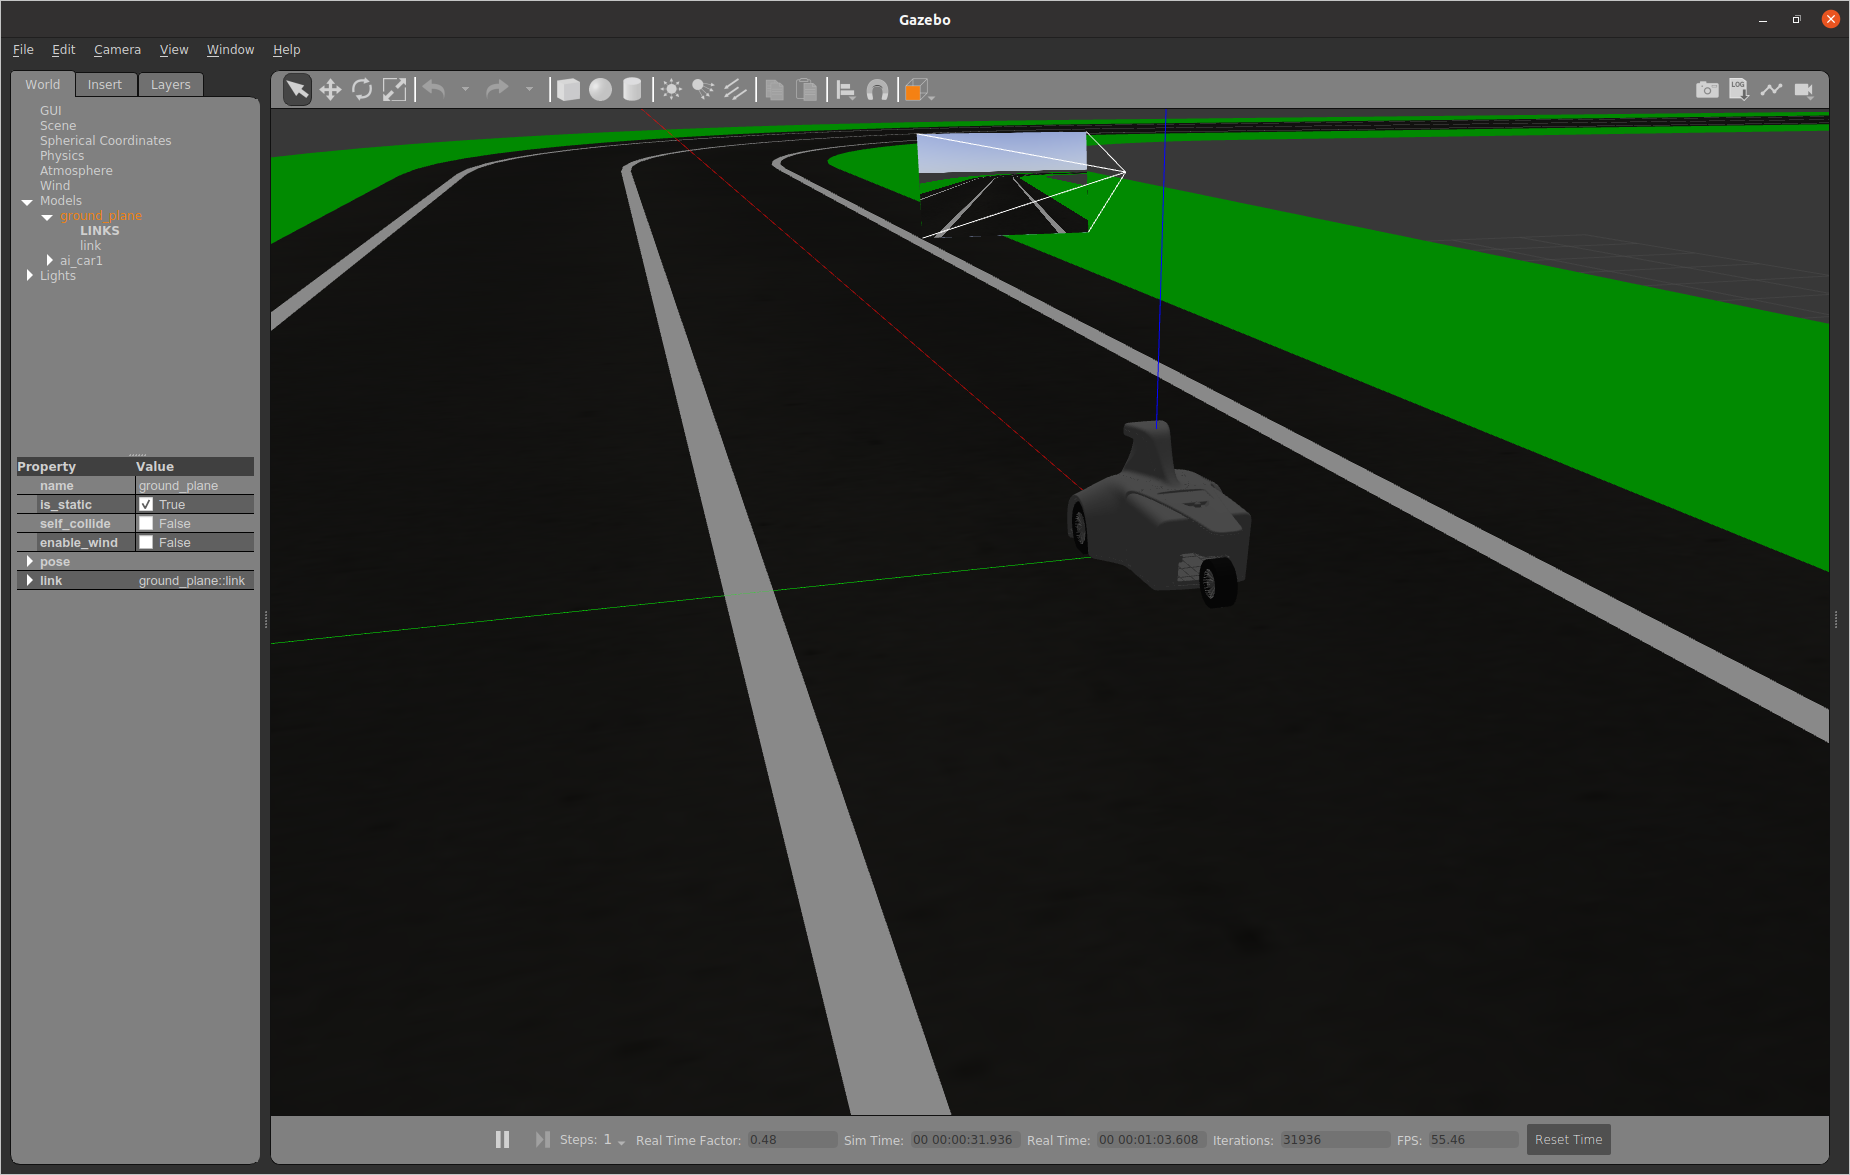
\includegraphics[keepaspectratio, scale=0.2]
      {images/simulator.png}
 \caption{Appearance of simulator}
 \label{fig:simulator}
\end{figure}

\begin{figure}[H]
  \centering
 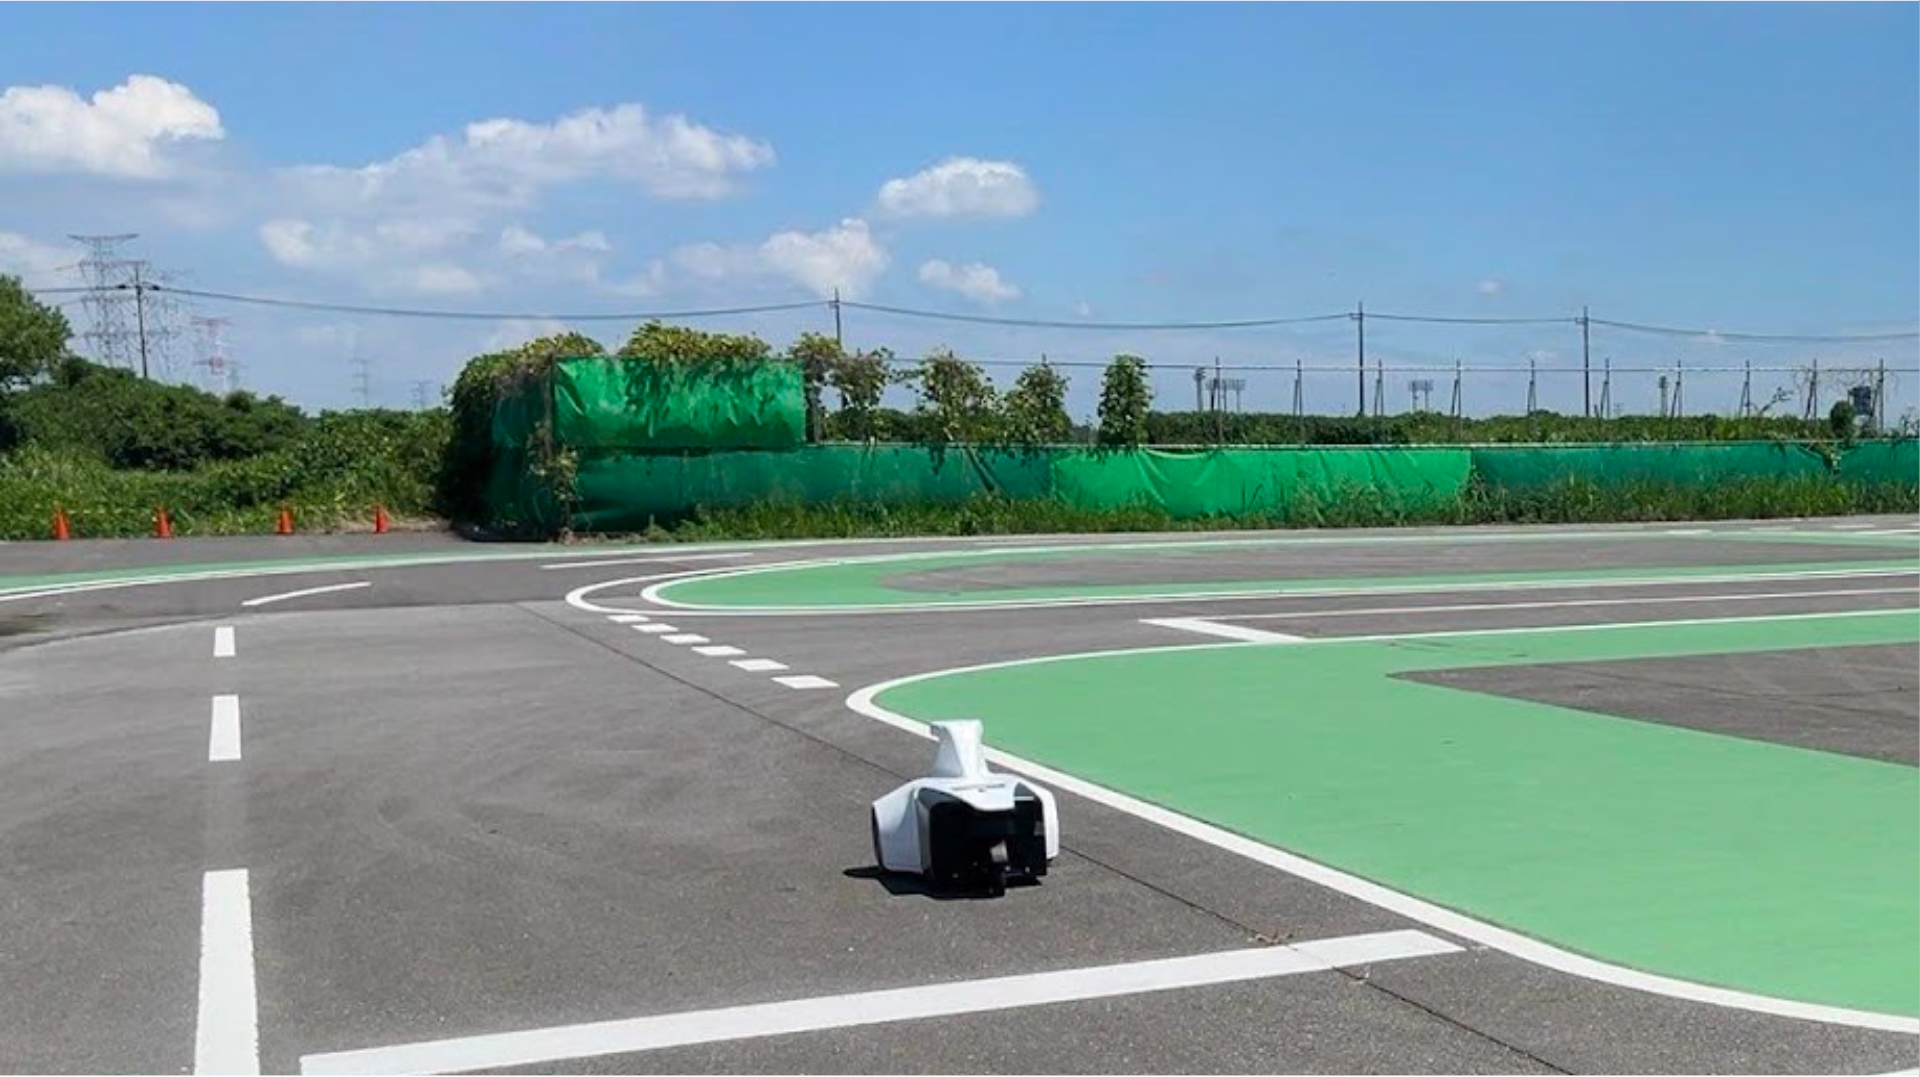
\includegraphics[keepaspectratio, scale=0.2]
      {images/realworld.png}
 \caption{AI-Formula and racing course}
 \label{fig:simulator}
\end{figure}

\newpage

% もっと前で議論ってどこ???
提供されたシミュレータ環境では基本的な機能が実装されているが, GNSS+IMUセンサ(VectorNav VN-200)の出力を再現できていない.
そのため, GNSS+IMUセンサ(VectorNav VN-200)の出力を再現する機能を追加して, 提供されたシミュレータを拡張して使用している.\cite{aifomrula-sim-chibakou}

シミュレータはROS 2とGazebo上で実装されており, Fig.5.3に示すようなノードの構成になっている.

\begin{figure}[H]
  \centering
 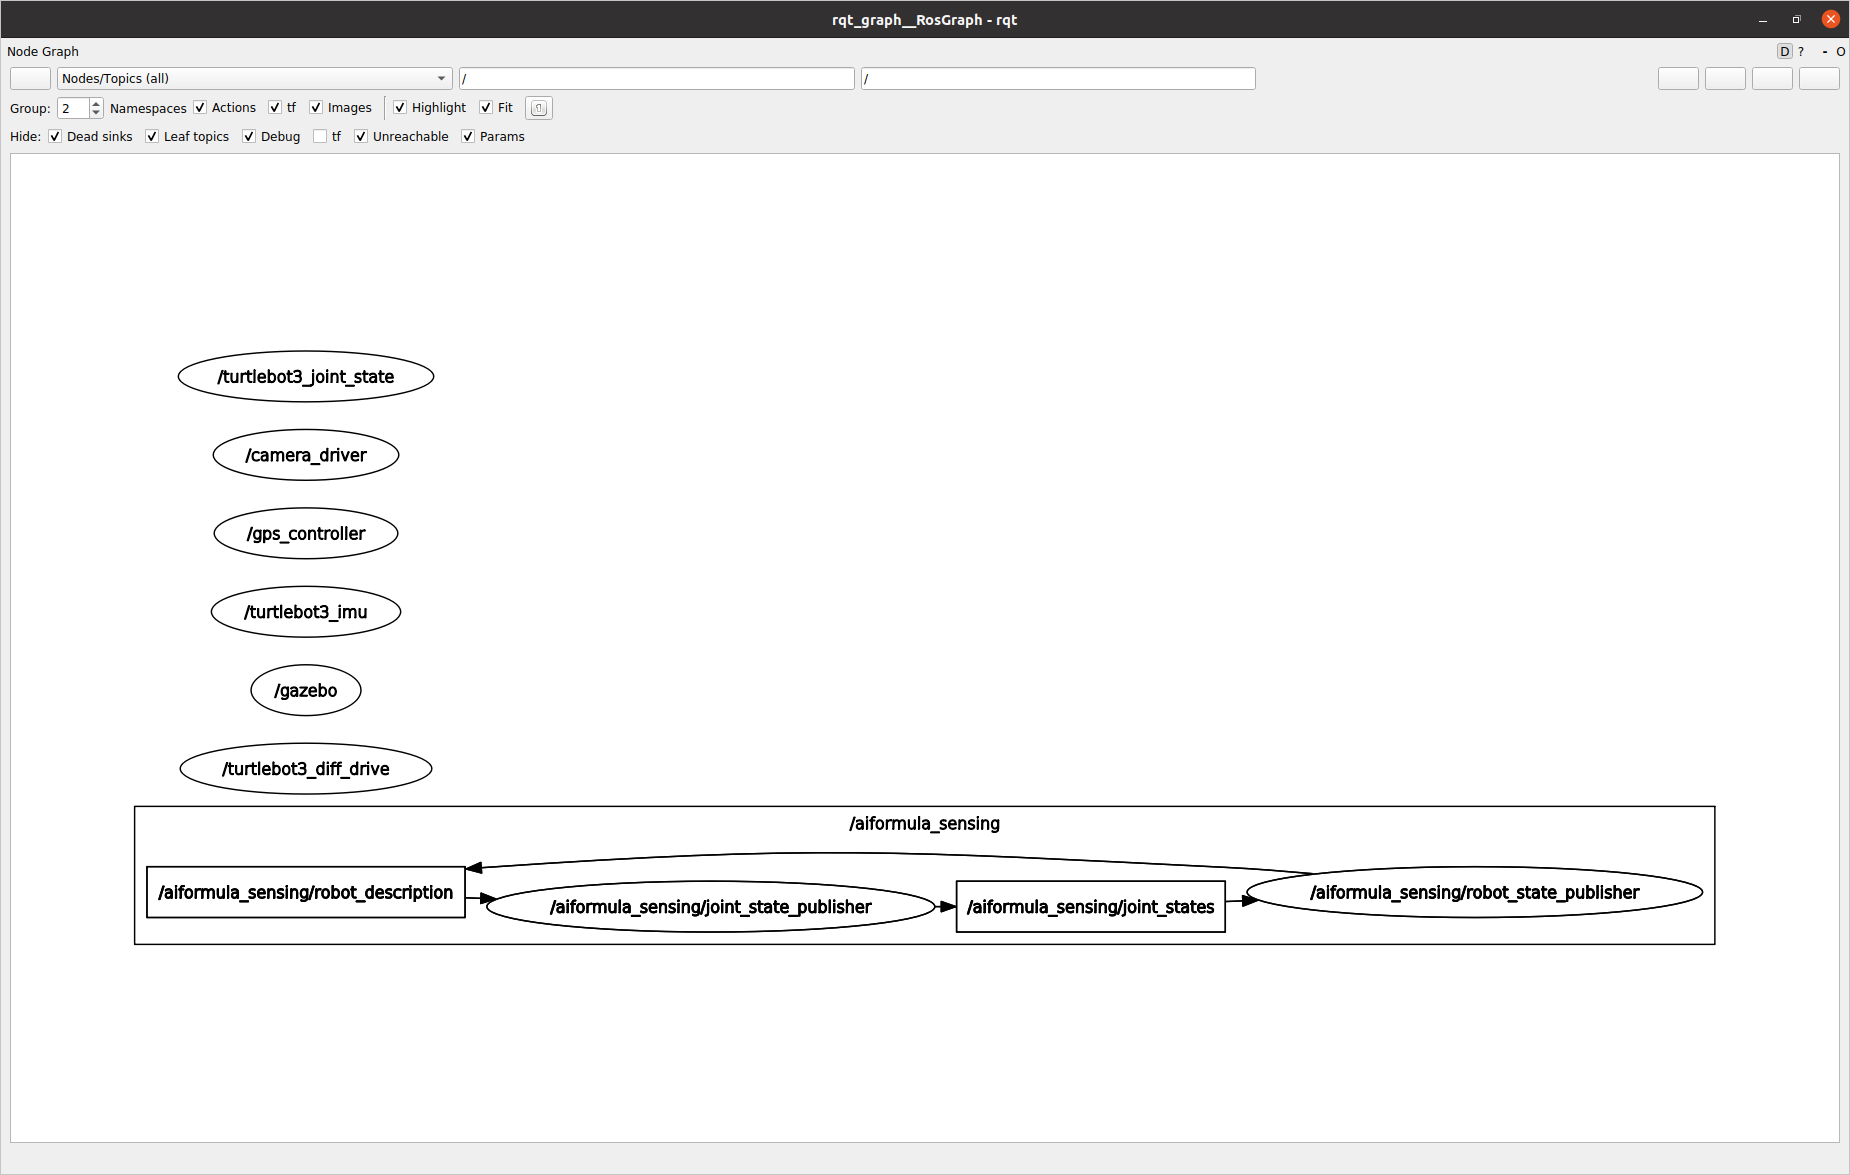
\includegraphics[keepaspectratio, scale=0.2]
      {images/rqt.png}
 \caption{Configuration of ROS 2 nodes}
 \label{fig:simulator}
\end{figure}

Table.5.1にシミュレーションする主なセンサとアクチュエータを示す.

\begin{table}[H]
  \centering
  \caption{Sensors and actuators to be simulated}
  \begin{tabular}{lclll}
  \cline{1-2}
  \multicolumn{1}{|l|}{}         & \multicolumn{1}{c|}{Camera}      &  &  &  \\
  \multicolumn{1}{|c|}{Sensor}   & \multicolumn{1}{c|}{IMU(Inertial Measurement Devices)} &  &  &  \\
  \multicolumn{1}{|l|}{}         & \multicolumn{1}{c|}{GNSS}        &  &  &  \\ \cline{1-2}
  \multicolumn{1}{|l|}{Actuator} & \multicolumn{1}{c|}{Drive motor} &  &  &  \\ \cline{1-2}
                                 & \multicolumn{1}{l}{}             &  &  & 
  % \caption{Sensors and actuators to be simulated}
  \end{tabular}
\end{table}

\section{実験の概要}
開発した経路追従ソフトウェアをシミュレータ環境で検証する.

\section{実験環境}
前述の提供されたシミュレータ環境にGNSS+IMUセンサ(VectorNav VN-200)の出力を追加したシミュレータ環境を使用する.
ソフトウェアにはROS 2 foxyを使用し, シミュレータ環境にはGazebo Classicを使用している.
Fig.5.4にシミュレータで扱うコースの全体図を示す.
Table.5.2にシミュレータに使用するPCの仕様を示す.

\begin{figure}[H]
  \centering
 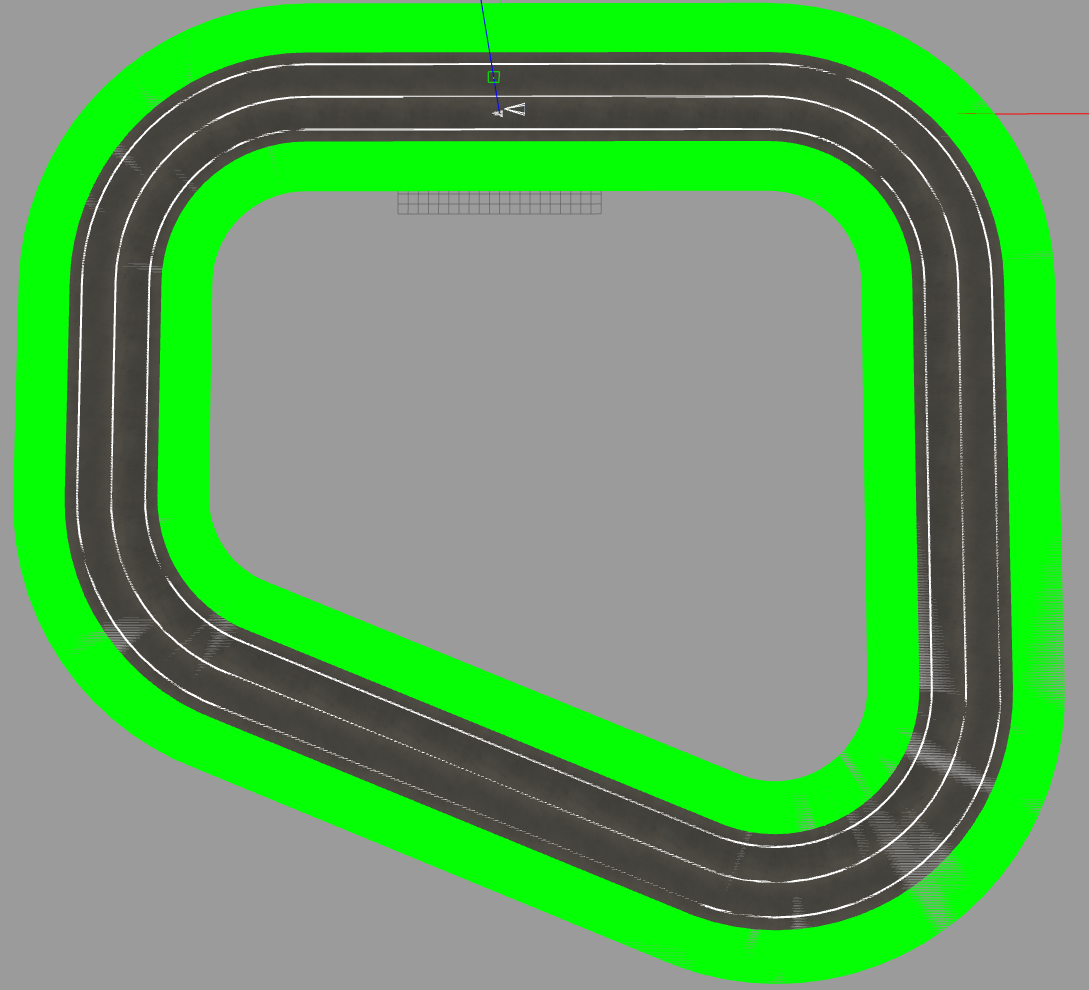
\includegraphics[keepaspectratio, scale=0.3]
      {images/topviewsim.png}
 \caption{Simulator world top view}
 \label{fig:simulator}
\end{figure}

\begin{table}[H]
  \centering
  \caption{experimental device}
  \begin{tabular}{cclll}
  \cline{1-2}
  Computer             & Let`s note CF-SV &  &  &  \\
  OS                   & Ubuntu20.04 LTS  &  &  &  \\
  ROS 2                & Foxy             &  &  &  \\
  simulator            & Gazebo Classic   &  &  &  \\
  \multicolumn{1}{l}{} &                  &  &  &  \\
  \multicolumn{1}{l}{} &                  &  &  & 
  \end{tabular}
\end{table}

\section{実験内容}
Fig5.5の丸で示された位置から矢印に沿うルートでシミュレータ環境のコースを一周させる.
制御パラメータは以下とし, 目標速度は一定値とする.

\begin{table}[H]
     \begin{tabular}{lcl}
         $目標速度$ & : & 6 [m/s] \\
         $制御周期$ & : & 20 [Hz] \\
     \end{tabular}
\end{table}
% 本実験では開発した経路追従ソフトウェアを前述のシミュレータ環境で検証する.
% 走行するコースをFig.5.5に示す.
% 本実験では予め決めたコースを1周したときのそれぞれの評価項目を確認することで作成した経路追従アルゴリズムの追従性の確認を行う.

\begin{figure}[H]
  \centering
 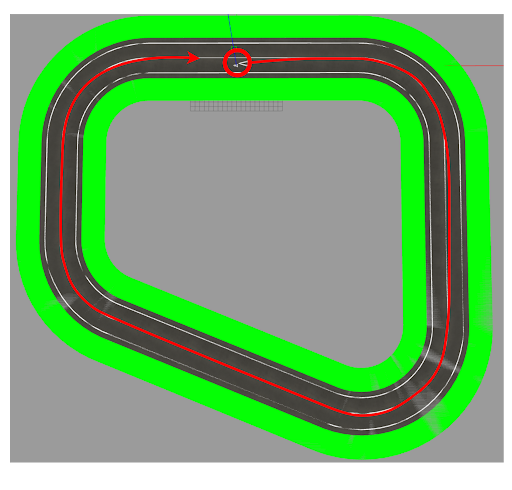
\includegraphics[keepaspectratio, scale=0.55]
      {images/simulatorpath.png}
 \caption{Simulator course}
 \label{fig:simulator}
\end{figure}

% \subsection{アルゴリズムの有効性を確認する実験}
% 作成した経路追従アルゴリズムの追従性を確認する実験を行う.
% 本実験では前述の通り予め決めたコースを1周させたときの評価項目や走行経路の軌跡から作成した経路追従アルゴリズムの有効性を判断する.

\section{実験結果}
シミュレータ環境で作成した経路追従ソフトウェアを使用することで実験を行った.

シミュレータで自律走行したときのロボットの軌跡をFig.5.6に示す.
結果として, シミュレータ環境のコースを周回することができた.

\begin{figure}[H]
  \centering
 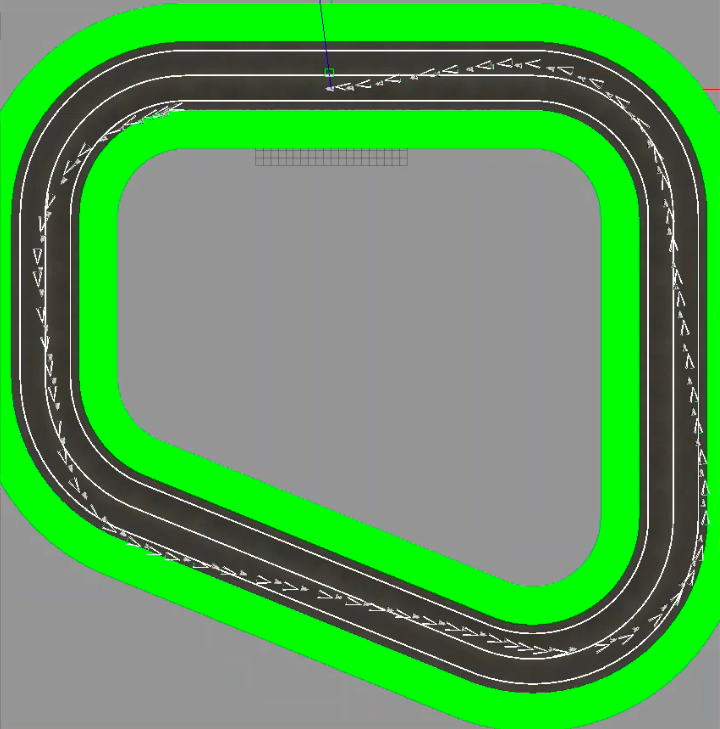
\includegraphics[keepaspectratio, scale=0.5]
      {images/simulatorfollowerpath.png}
 \caption{The AI-Formula path-following behavior on the simulator}
 \label{fig:simulatorpath}
\end{figure}